\documentclass[a4paper,10pt]{report}
\usepackage[utf8]{inputenc}
\usepackage{tikz}
\usepackage[fleqn]{amsmath}

\begin{document}
Just a short explanation how the calculations for the graver sharpening jig works. 
Normally, there are three 5 parameters that define the form of the base plate:


\begin{tabular}{ll}
 $\alpha$ & Angle of the cutting face \\
 $\beta$ & Angle of the v-shape \\
 $\theta$ & Angle of the heel \\
 $d$ & Elevation of the sharpening stone over the plane the jig is running on \\
 $s$ & Stick out, the length the graver is protruding from the front face of the jig
\end{tabular} 


\vspace{2em}
In order to print a jig with a given width $b$, three main dimensions are calculated:
\vspace{1em}

\begin{minipage}{0.45\textwidth}
 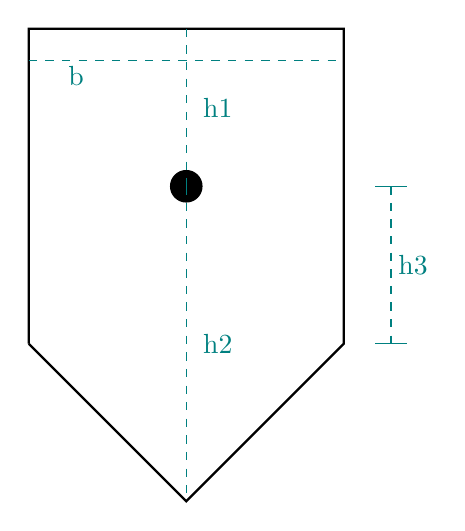
\begin{tikzpicture}[scale=2]
\draw[thick] (0,0) -- (0,2)-- (2,2) -- (2,0) -- (1,-1) -- (0,0);
\draw [fill] (1,1) circle [radius=0.1];

\draw[teal, dashed] (0,1.8) -- (2,1.8);
\node[teal] at (0.3,1.7) {b};

\draw[teal, dashed] (1,2) -- (1,1);
\node[teal] at (1.2,1.5) {h1};

\draw[teal, dashed] (1,1) -- (1,-1);
\node[teal] at (1.2,0) {h2};

\draw[teal] (2.2,1) -- (2.4,1);
\draw[teal] (2.2,0) -- (2.4,0);
\draw[teal, dashed] (2.3,1) -- (2.3,0);
\node[teal] at (2.44,0.5) {h3};
\end{tikzpicture}
\end{minipage}
\begin{minipage}{0.45\textwidth}
 \begin{tabular}{lp{5cm}}
  $h1$ & Distance between the axis of the graver and the edge of the jig (for face sharpening) \\
  $h2$ & Distance between the axis of the graver and the tip of the jig (for the heels) \\
  $h3$ & Height from graver axis to the lower corners (for the heels) \\
 \end{tabular}
\end{minipage}

With some base geometry the dimensions can be found to be:
$$
    h_1 = \frac{s \cdot \sin \alpha  + d}{\cos \alpha}
$$
$$
    h_2 = \frac{s \cdot \sin \theta  + d}{\cos \theta \cdot \sin \frac{\beta}{2}}
$$
$$
    h_3 = h_2 - \frac{b}{2 \tan \frac{\beta}{2}}
$$

\section*{Example (distances in mm, angles in °):}
\begin{minipage}{0.65\textwidth}
given: \\
$b=50, d=20, s=30$ \\ $\alpha=45, \beta=105, \theta=8 $
$$
    h_1 = \frac{30 \cdot \sin 45  + 20}{\cos 45} \approx \frac{41.2}{0.71} \approx 49.5
$$
$$
    h_2 = \frac{30 \cdot \sin 8  + 20}{\cos 8 \cdot \sin 52.5} \approx \frac{24.2}{0.8} \approx 30.8
$$
$$
    h_3 = 30.8 - \frac{25}{\tan 52.5} \approx 11.6
$$

\end{minipage}
\begin{minipage}{0.25\textwidth}
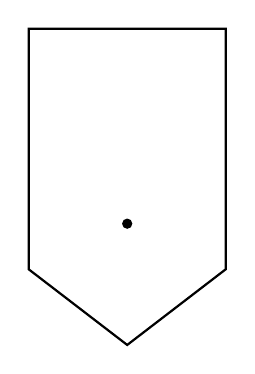
\begin{tikzpicture}[scale=0.05]
\draw[thick] (0,0) -- (0,49.5) -- (50,49.5) -- (50,0) -- (50,-11.6) -- (25,-30.8) -- (0,-11.6) -- (0,0) ;
\draw [fill] (25,0) circle [radius=1.15];
\end{tikzpicture}
\end{minipage}









\end{document}
